\chapter{Event Selection}
\label{chap:EventSelection}

\noindent From an hypothetical \Zprimetotauh~decay, both taus would 
be oppositely charged, highly boosted and would travel 
in opposite directions. Due to the presence of neutrinos in 
the tau decay, a missing transverse energy requirement
is applied to reduce the QCD contamination. Additionally, 
in order to reduce the \ttbar~contamination, a b-jet veto 
is required. All these topological signal selections are summarized 
as:

\begin{itemize}
  \item \MET $>$ 30 \GeV.
  \item $\#$ b-jets (CSVv2 Loose WP) $= 0$.
  \item $Ch_{\tau_{1}} \times Ch_{\tau_{2}} <$ 0.
  \item \DRt $>$ 0.3.  
  \item $\cos\Delta \phi (\tau_{1},\tau_{2}) <$ -0.95.
 \end{itemize}

\noindent However, since the neutrinos coming from the hadronic tau decays are expected 
to be very energetic and, therefore, collinear to the tau decay products, there is a 
complex relation between the direction of the hadronic taus and the direction of 
the missing transverse energy. With the purpose to identify the optimal cut 
that accounts for such complex relation and, that discriminates better 
between signal and background, the significance was computed for 
several topological variables that have been used 
in previous di-tau final state searches. Table \ref{tab:EventSelection} shows 
the variables considered for the selection optimization.

{\renewcommand{\arraystretch}{1.5}%  
\begin{table}[H]
% \scalebox{1.5}{a}
\begin{center}
\resizebox{\textwidth}{!}{
 \begin{tabular}{|l|c|c|}  \hline \hline 
  Label in plot                      & Color in plot & Selections \\ [.5ex] \hline \hline
  CosDphi\_LeadingTauAndMET          & blue   & $\cos\Delta \phi (\tau_{lead},\not\!\!E_T) < -0.9$ \\ [.5ex] \hline
  pZeta                              & green  & $p_{\zeta}- 3.1 \times p_{\zeta}^{vis} > -50~$\GeV    \\ [.5ex] \hline
  \multirow{2}{*}{\shortstack[l]{Cos\_Tau1AndMET\_OR\_CosTau2AndMET}} &   \multirow{2}{*}{\shortstack[c]{purple}} & $\cos\Delta \phi (\tau^{lead}, \not\!\!E_T) < -0.9$ or  \\ [.5ex]
                                                                      &                                           & $\cos\Delta \phi (\tau_{2}, \not\!\!E_T) < -0.9$ \\ [.5ex] \hline
  Rate                               & orange & $ -1.05 < \frac{\cos\Delta \phi (\tau^{lead},~\not\!\!E_T)}{\cos\Delta \phi (\tau_{2},~\not\!\!E_T)}  < -0.95$   \\ [.5ex] \hline
  \end{tabular}
  }
\end{center}
\caption{Selections considered. \label{tab:EventSelection}}
\end{table}
}
 
\noindent The variables of the pZeta cut are defined as:

\begin{equation}
   p_{\zeta}^{vis} = \overrightarrow{p}_{\tau_{1}}^{vis}\hat{\zeta}+\overrightarrow{p}_{\tau_{2}}^{vis}\hat{\zeta} \; ,
\label{eq:zetavis}
\end{equation}
\begin{equation}
   p_{\zeta} = p_{\zeta}^{vis}+\overrightarrow{{E\!\!\!\!/_{\rm T}}}\hat{\zeta} \; ,
\label{eq:zeta}
\end{equation}

\noindent where $\hat{\zeta}$ is the unit vector along the bisector of the visible tau decay products,
$p_{\zeta}^{vis}$ and $p_{\zeta}$ are two projection variables on the $\hat{\zeta}$ direction. The pZeta 
selection was used in the search for \Zprime~bosons in the di-hadronic channel,
performed with the data collected during 2015 \cite{CMSZprimetotautau2015}. \\

\noindent The signal yield and the total background were estimated using 
the same procedure described in Chapter \ref{chap:Analysis}. Figure \ref{fig:EventSelection} shows 
the comparison among the significances (as a function of the 
effective visible mass) obtained with each topological cut 
considered. The significance was computed for several \Zprime~mass points. Note 
in the figure that the highest significance is obtained with 
the $\cos\Delta \phi (\tau_{lead},\not\!\!E_T) < -0.9$ cut; therefore, 
this cut was selected for the analysis presented in this work.

\begin{figure}[ht]
\begin{center}
\captionsetup[subfloat]{farskip=0pt,captionskip=0.0cm,labelformat=empty}
\resizebox{\textwidth}{!}{
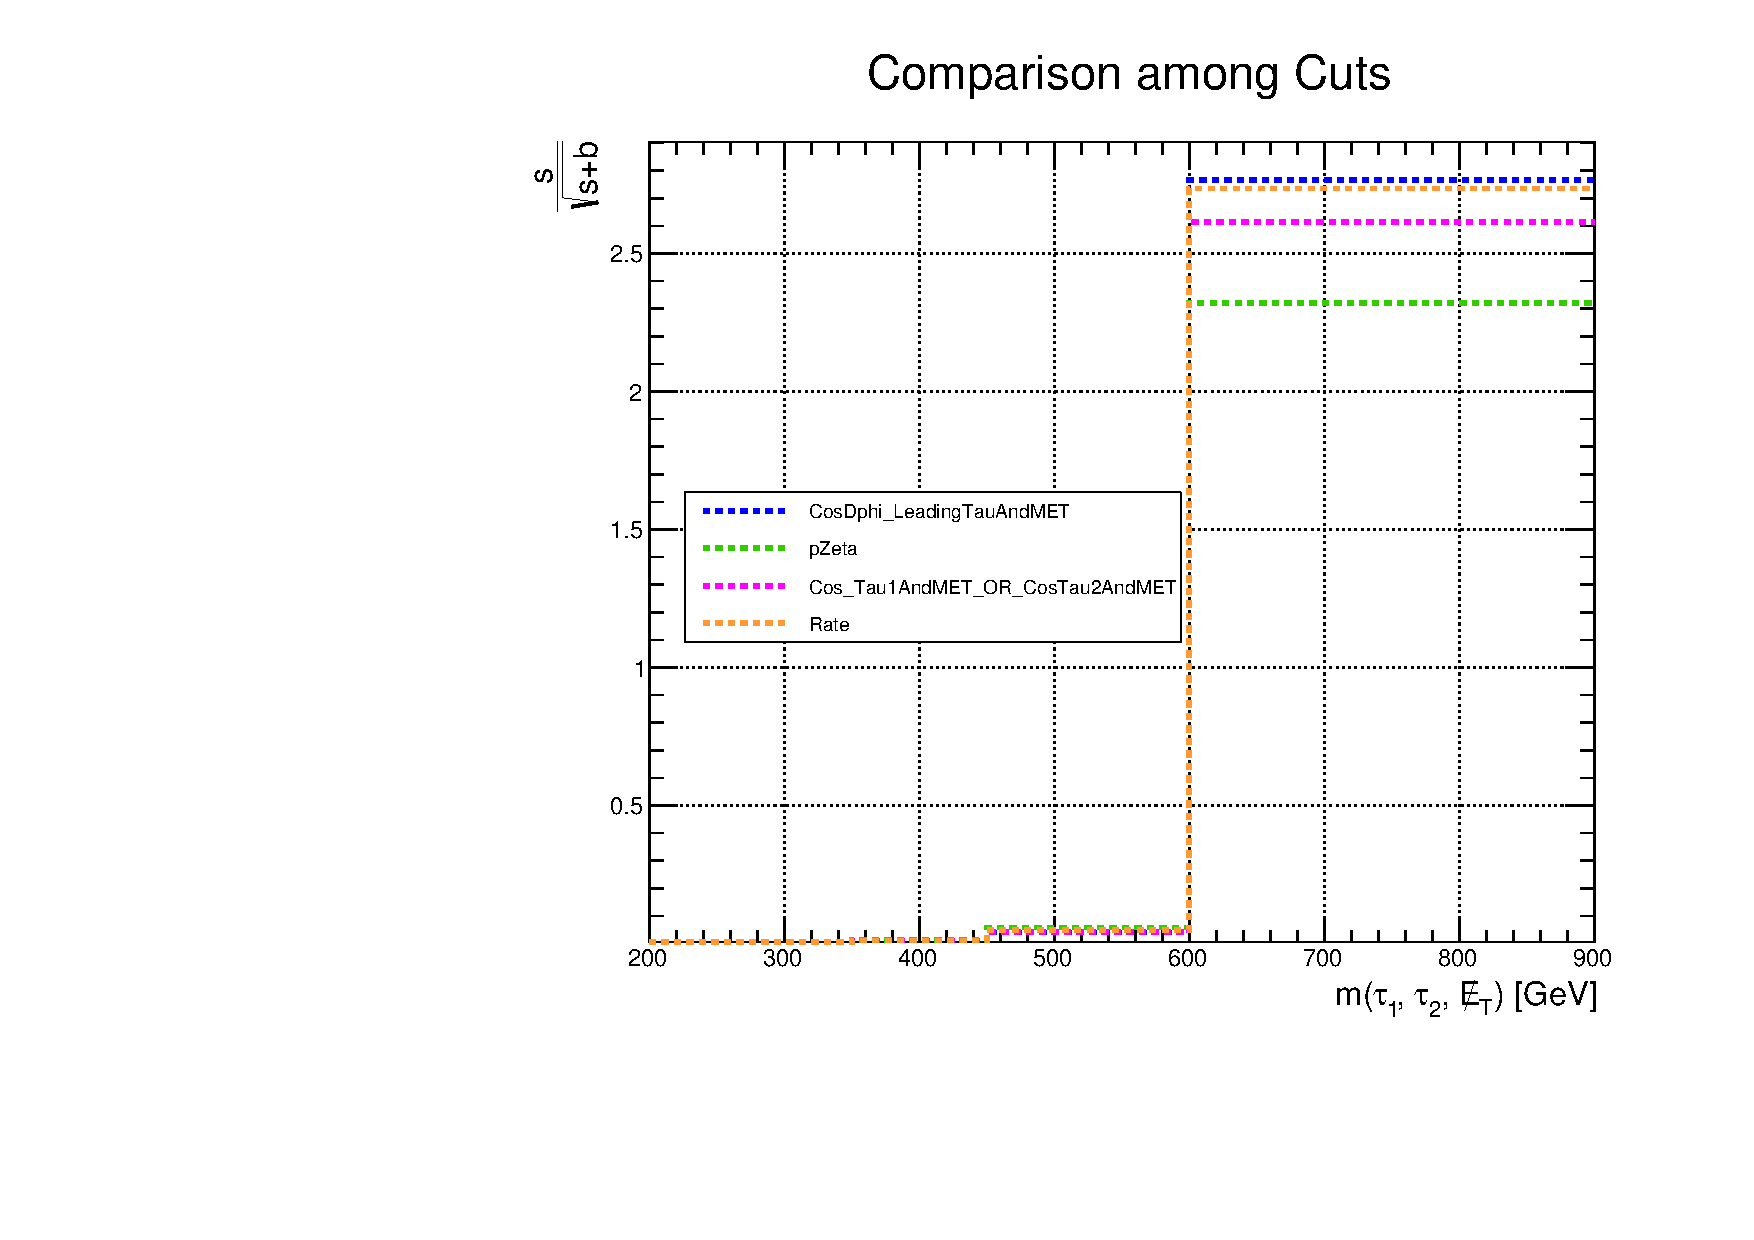
\includegraphics[clip,width=0.46\textwidth]{figuras/AppendiceC/Zprime2000.pdf}
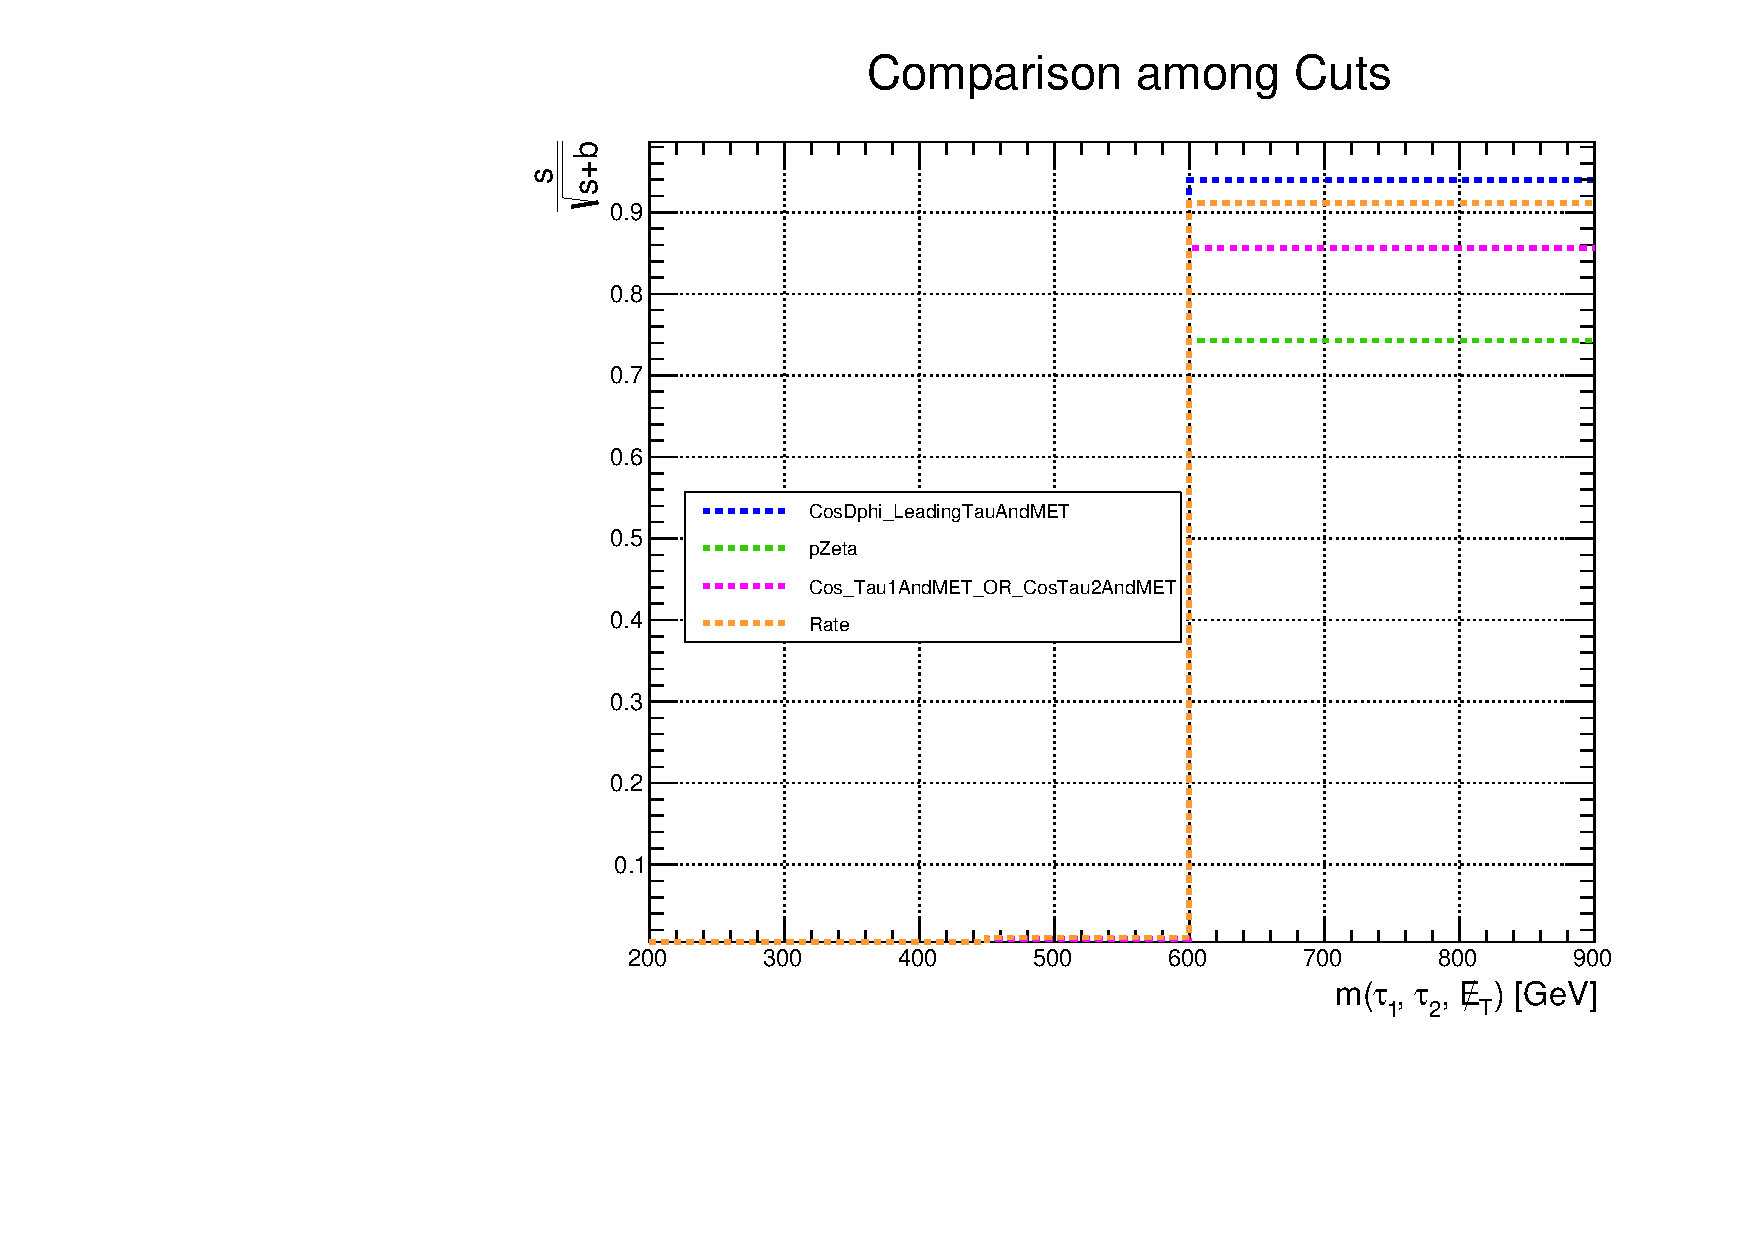
\includegraphics[clip,width=0.46\textwidth]{figuras/AppendiceC/Zprime2500.pdf}
}
\resizebox{\textwidth}{!}{
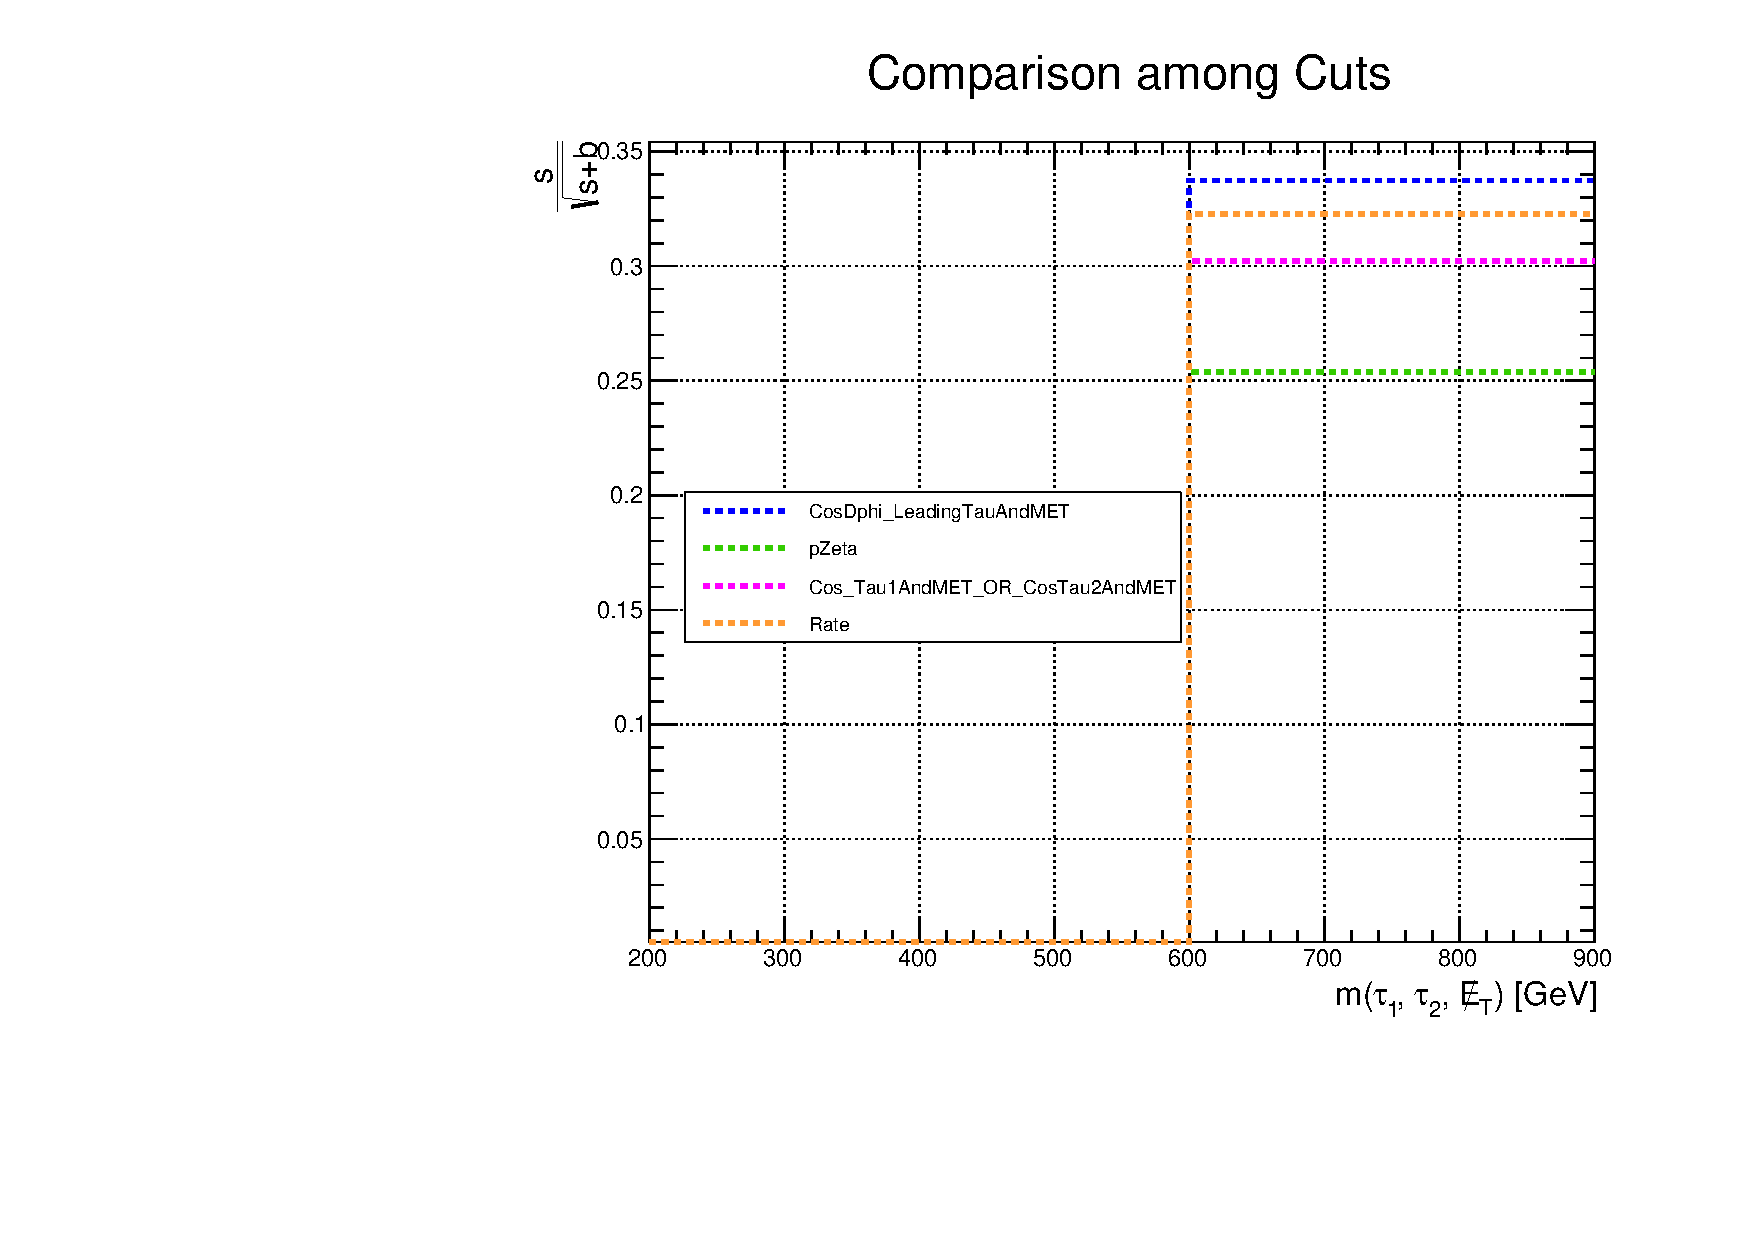
\includegraphics[clip,width=0.46\textwidth]{figuras/AppendiceC/Zprime3000.pdf}
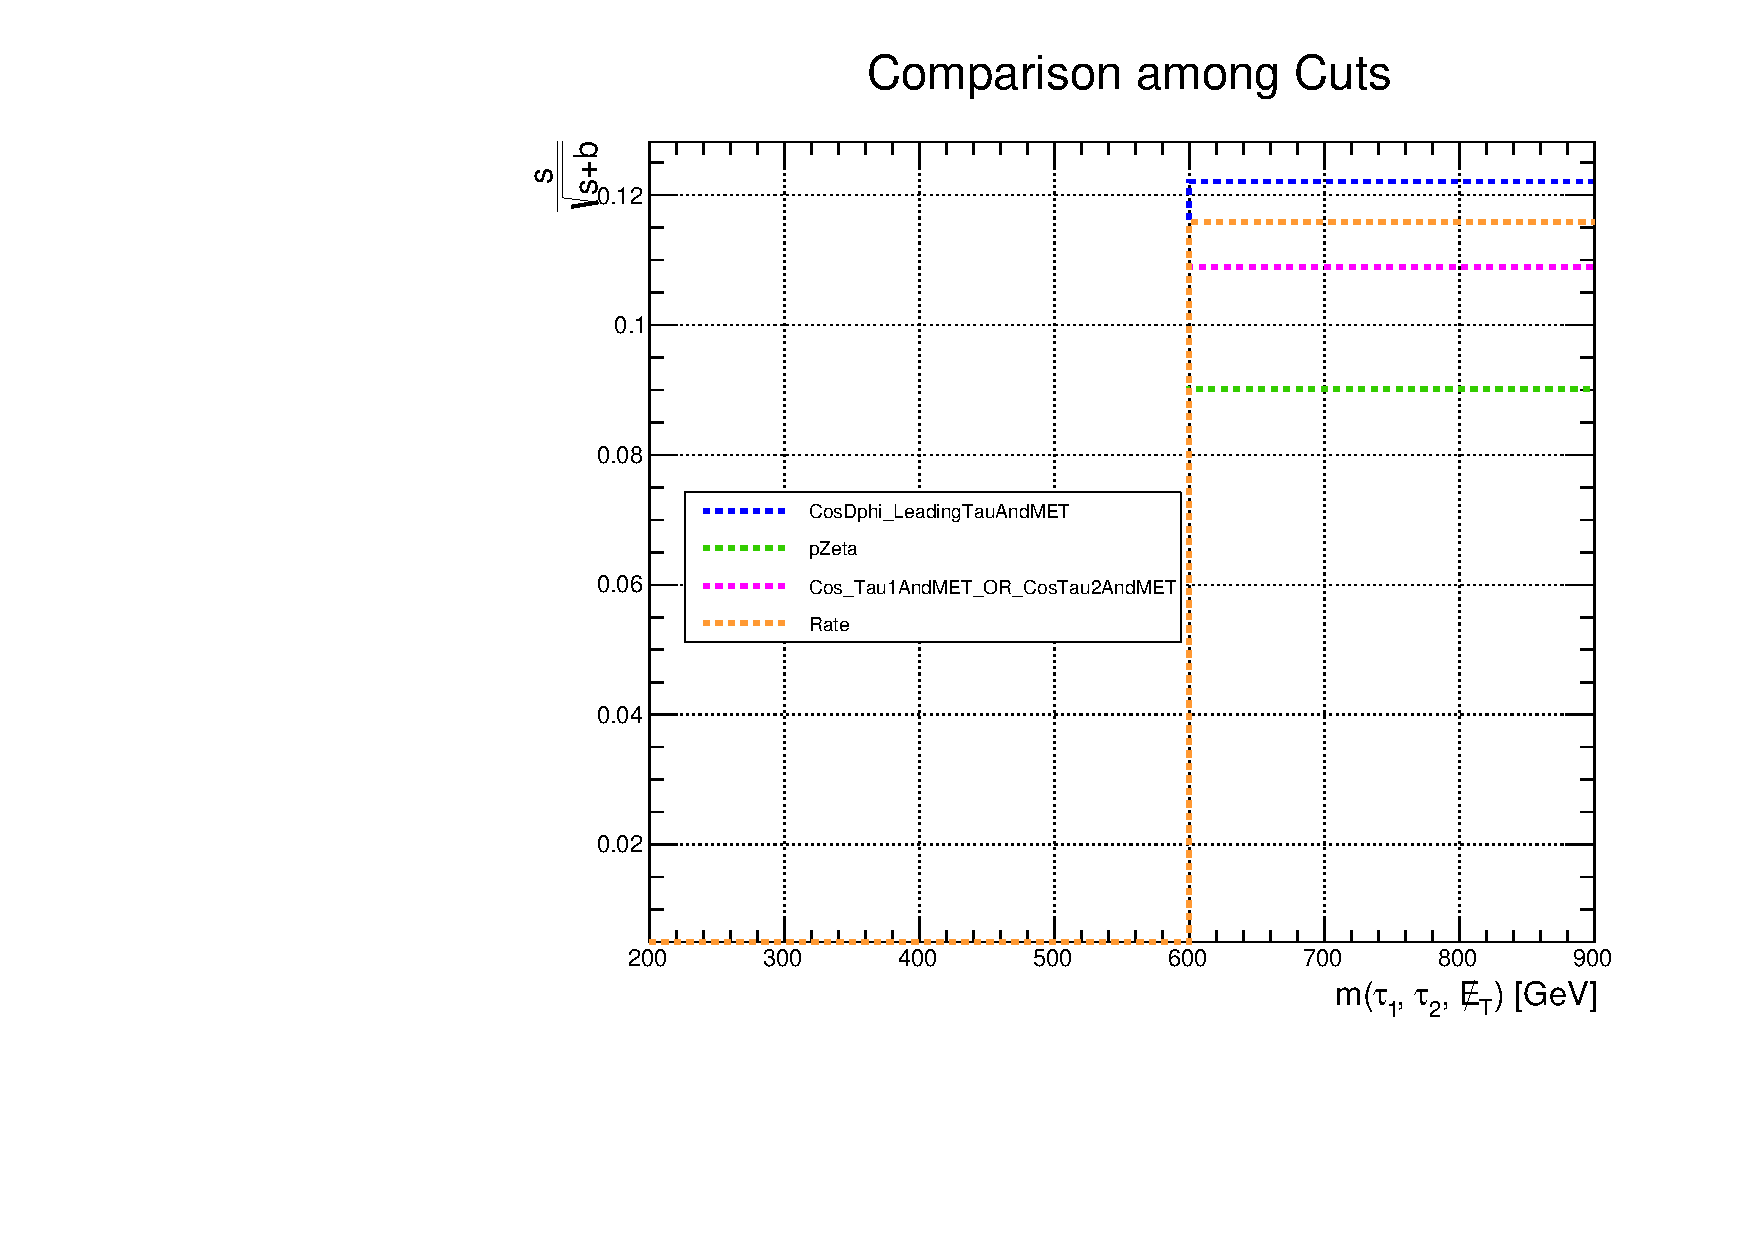
\includegraphics[clip,width=0.46\textwidth]{figuras/AppendiceC/Zprime3500.pdf}
}
\caption{Significance, as a function of the effective visible mass, obtained 
with different selections after requiring \MET $>$ 30 \GeV, b-jet veto (CSVv2 Loose WP),
$Ch_{\tau_{1}} \times Ch_{\tau_{2}} <$ 0, \DRt $>$ 0.3 and 
$\cos\Delta \phi (\tau_{1},\tau_{2}) <$ -0.95. Significance computed 
with a \Zprime~masses of 2000 \GeV (top left), 2500 \GeV (top right),
3000 \GeV (bottom left) and 3500 \GeV (bottom right). \label{fig:EventSelection}}
\end{center}
\end{figure}